\section{Results}

\subsection{Baselines $\&$ Comparisons}

The first baseline is the combination of reinforcement learning and hindsight experience replay. The combination of DDPG+HER when proposed was able to achieve much success in solving complex multi-goal robotics tasks and has set a benchmark for future research to come. This is an environmental baseline and was the first to solve sparse reward environments used in this research and will be used to compare the current implementation's capability to solve the environment successfully. \\

The second baseline is much closer to this research in terms of algorithm and implementation also combining behavior cloning with reinforcement learning. DDPG+BC along with expert demonstrations was able to successfully accelerate complex robotics tasks in the mentioned environments. This is an algorithmic baseline that was first provided accelerated learning for the environments used in this research and will be used to compare the current implementation's capability to further provide accelerated learning. \\

The third baseline implements pure behavior cloning using demonstrations and will serve as a comparison for why this method has either great or really poor performance. \\

The fourth baseline implements plain reinforcement learning without demonstrations or hindsight experience replay but with dense rewards and was able to achieve good performance in accelerating complex multi-goal robotics tasks. This is a reward baseline that first proposed a new reward function for the multi-goal robotic sparse reward environments used in this research and will be used to compare the current implementation's capability to provide accelerated learning. \\

Apart from comparison with the baselines, there will be other comparisons as well, first with the current implementation itself but with a different demonstration source. The main reason for this comparison is if the current framework implementation is kept fixed while varying different sources of demonstrations, will there be any impact on the performance of the algorithm. Second, there will be a comparison between the generalization capabilities between the current implementation and baseline 1 to check if after the training phase the agent can perform well in the testing phase as well. The third will be a short comparison between the network complexity used between the current implementation and baseline 2 to see if the acceleration comes at a cost of model complexity, also this being very similar approaches the number of demonstrations used will also be compared to see if good performance can be achieved using lesser number of demonstrations. Finally, there will be a comparison between the hardware used and training time for the current implementation and baselines 2, 4 to see if the current implementation can strike a balance between the training time and hardware resources used. \\

The comparison between the current implementation and the baselines will take place in terms of task success rate. The success rate is calculated during the testing phase of the training runs and if the agent can successfully end the episode with a successful task completion then the success rate for that agent is incremented. The baselines calculate the success rate by performing 10 deterministic roll-outs per worker and then calculate the average per test set then averaged across all the workers. One of the main advantages of the current implementation is that it does not require multi-processing or parallel implementations with parallel workers like the baselines and uses just one worker with one roll-out test set from which the average success rate is calculated. The plot represented the average success rate of the test run set during the training phase and the performance will be determined by how soon the agent can achieve the highest possible success rate for a given task. Further comparisons will be in terms of training times vs hardware complexity and model complexity. \\

For task 1 the current implementation will be compared to only baseline 1, baselines 2 and 3 are not available for comparison due to the comparatively simple nature of the environment it was not implemented as a part of this baseline research, but in this paper results for the current implementation is presented for this environment to stay consistent across all the environments in the fetch robotics environment suite. For tasks 2 and 3 the current implementation will be compared with baselines 1, 2 and 3. Baseline 4 will be used only for task 4 as that research only focuses on this particular environment. The comparison between different sources of demonstrations will also be done only for task 4 due to the use of a handcrafted script as a different source of demonstration. This script was not developed as a part of this research and was provided by the baselines team \cite{stable-baselines} as an example for this particular environment. \\

Some abbreviations used in the results to denote the number of time steps are, K and M which corresponds to 1 Thousand and 1 Million respectively. All the graphs and visualizations seen in this research was captured using the Weights and Biases toolbox \cite{wandb}. \\

\subsection{Fetch Reach Environment}

\begin{figure}[h!]
     \centering
     \begin{subfigure}[b]{0.4\textwidth}
         \centering
         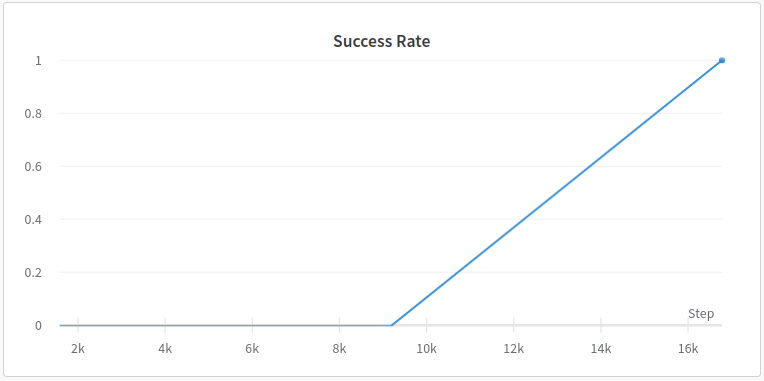
\includegraphics[width=\textwidth]{images/FRSR.png}
         \caption{Success Rate Plot of the Current Implementation.}
     \end{subfigure}
     \begin{subfigure}[b]{0.4\textwidth}
         \centering
         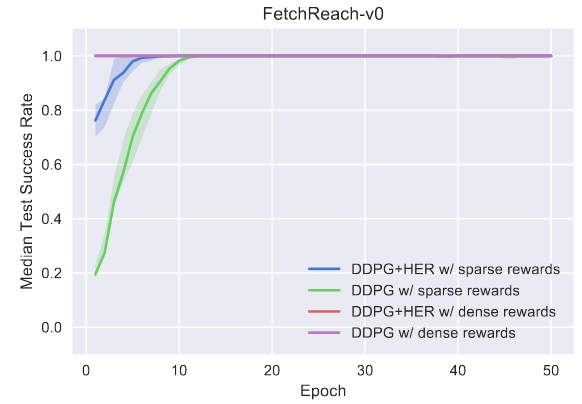
\includegraphics[width=\textwidth]{images/FRB.png}
         \caption{Success Rate Plot for Baseline 1 \cite{andrychowicz2018hindsight}.}
     \end{subfigure}
        \caption{Comparison Between Current Implementation and Baseline 1 for Fetch Reach Task, Epoch Number (every epoch = 800 episodes = 800x50 time steps).}
        \label{fig:FRR}
\end{figure}

In the fetch reach environment, compared to baseline 1, the current implementation has a much higher convergence rate. Figure \ref{fig:FRR} shows the current implementation can reach a success rate of 1.0 at approximately 16K time steps whereas baseline 1 reaches the same success rate of 1.0 at approximately 150K time steps. Not only does the current implementation solve the task successfully but also provides accelerated learning for this environment. \\

\subsection{Fetch Push Environment}

\begin{figure}[h!]
     \centering
     \begin{subfigure}[b]{0.4\textwidth}
         \centering
         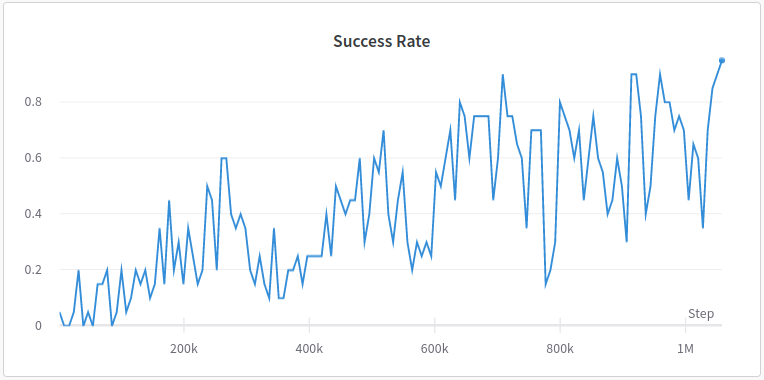
\includegraphics[width=\textwidth]{images/FPSR.png}
         \caption{Success Rate Plot of the Current Implementation.}
     \end{subfigure}
     \begin{subfigure}[b]{0.4\textwidth}
         \centering
         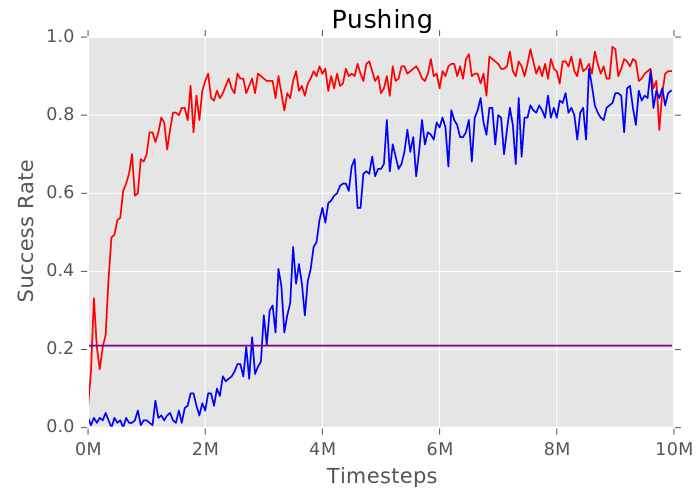
\includegraphics[width=\textwidth]{images/FPB.png}
         \caption{Success Rate Plot for \textcolor{blue}{Baseline 1}, \textcolor{red}{Baseline 2}, \textcolor{violet}{Baseline 3} \cite{nair2018overcoming}.}
     \end{subfigure}
        \caption{Comparison Between Current Implementation and Baselines 1, 2 and 3 for Fetch Push Task.}
        \label{fig:FPR}
\end{figure}

In the fetch push environment, baseline 3 performs the worst by achieving a success rate of only 0.2, performing similar or worse than a random agent. Baseline 1 can successfully solve the environment and reaches a success rate of 0.8 in 10M time steps and baseline 2 can beat it by reaching a success rate of 0.9 in 3M time steps and a success rate of 0.95 in 6M time steps. Figure \ref{fig:FPR} shows that the current implementation can beat all the previous baselines by reaching a success rate of 0.95 in approximately 1.1M time steps, solving the environment successfully and also providing accelerated learning. An interesting observation here is that the demonstrations used had a clear pushing motion where the end effector of the robot arm is used to push the block towards the goal. However, the final agent learned behavior is slightly different from what is expected. The agent can use the end effector of the robot arm to successfully move the object to the goal, but instead of a pushing motion, it uses a poking motion. The main reason could be the dynamics of the environment, MuJoCo uses a soft body collision system for its interactions. This might have influenced the agent to interact differently with the objects in the environment. Even though the goal might be successful, this particular motion might not be a desirable behavior for real-world applications. This can easily be fixed by changing the constraints to rigid body collisions, but this was not done for this research as this process increases the simulation time of the environment significantly. But one positive outcome is that the agent in the current implementation is not bound or constrained to the actions of the demonstrations, it can modify its actions as per the environment and develop new behaviors. As an extension to this research, it would be interesting to try out two things, in the same environment try to use rigid body collisions and then observe the new behavior or try to find a way to overcome the soft body constraints and develop a usable behavior. \\

\subsection{Fetch Slide Environment}

\begin{figure}[h!]
     \centering
     \begin{subfigure}[b]{0.4\textwidth}
         \centering
         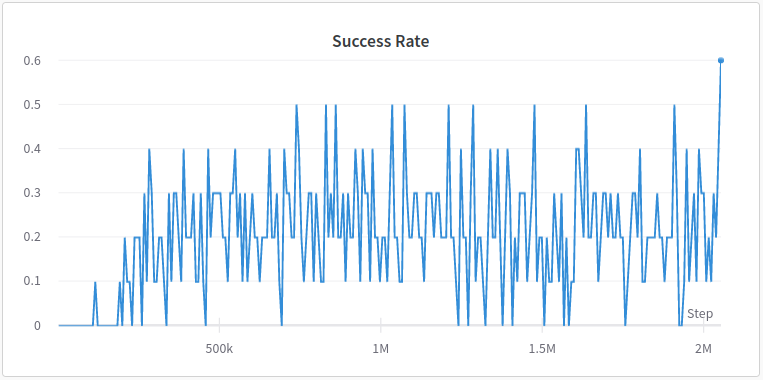
\includegraphics[width=\textwidth]{images/FSSR.png}
         \caption{Success Rate Plot of the Current Implementation.}
     \end{subfigure}
     \begin{subfigure}[b]{0.4\textwidth}
         \centering
         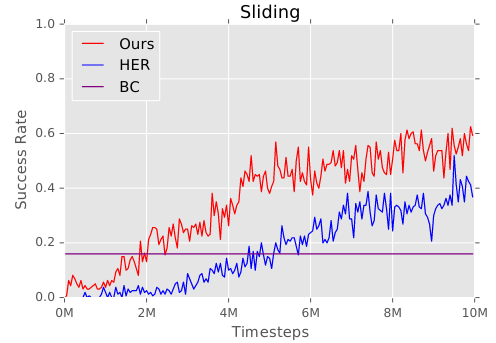
\includegraphics[width=\textwidth]{images/FSB.png}
         \caption{Success Rate Plot for \textcolor{blue}{Baseline 1}, \textcolor{red}{Baseline 2}, \textcolor{violet}{Baseline 3} \cite{nair2018overcoming}.}
     \end{subfigure}
        \caption{Comparison Between Current Implementation and Baselines 1, 2 and 3 for Fetch Slide Task.}
        \label{fig:FSR}
\end{figure}

The fetch slide is the most complex environment of the suite and that is evident by looking at figure \ref{fig:FSR}. Baseline 3 fails this environment as well and achieves a success rate of only 0.2, very similar to the fetch push environment. The baseline 1 can solve the environment but the performance is poor with a success rate of 0.4 in 10M time steps. Both the baseline 2 and current implementation can solve the environment as well and both reach a respectable success rate of 0.6, the baseline 2 can do this in 10M time steps whereas the current implementation can achieve it in just 2M time steps showing a successful acceleration in learning. As an extension to this research, it would be interesting to see whether the current implementation if trained for longer will be able to achieve a higher success rate. \\

\subsection{Fetch Pick and Place Environment}

\begin{figure}[h!]
     \centering
     \begin{subfigure}[b]{0.4\textwidth}
         \centering
         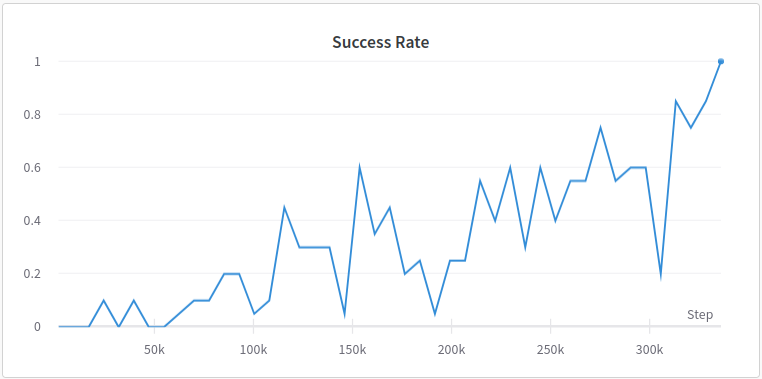
\includegraphics[width=\textwidth]{images/FPAPASR.png}
         \caption{Success Rate Plot of the Current Implementation.}
     \end{subfigure}
     \begin{subfigure}[b]{0.4\textwidth}
         \centering
         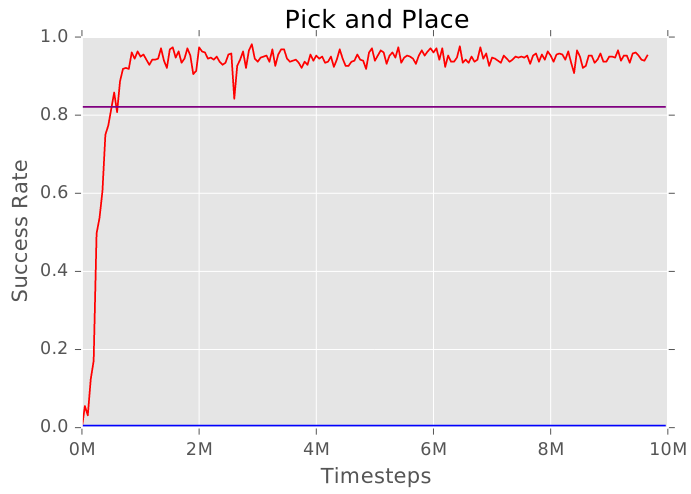
\includegraphics[width=\textwidth]{images/FPAPB.png}
         \caption{Success Rate Plot for \textcolor{blue}{Baseline 1}, \textcolor{red}{Baseline 2}, \textcolor{violet}{Baseline 3} \cite{nair2018overcoming}.}
     \end{subfigure}
        \caption{Comparison Between Current Implementation and Baselines 1, 2 and 3 for Fetch Pick and Place Task.}
        \label{fig:FPAPR1}
\end{figure}

\begin{figure}[h!]
     \centering
     \begin{subfigure}[b]{0.5\textwidth}
         \centering
         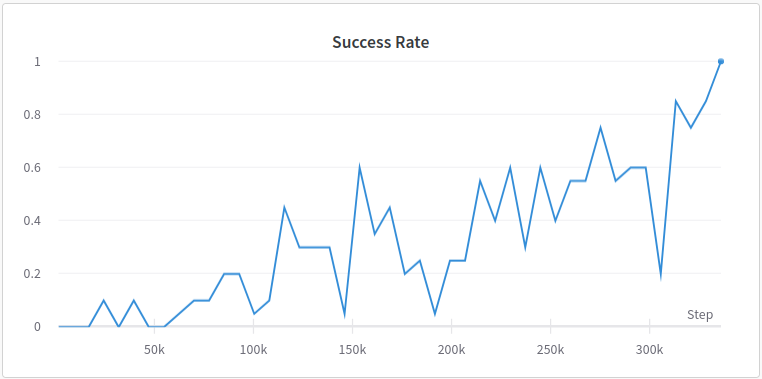
\includegraphics[width=\textwidth]{images/FPAPASR.png}
         \caption{Success Rate Plot of the Current Implementation.}
     \end{subfigure}
     \begin{subfigure}[b]{0.5\textwidth}
         \centering
         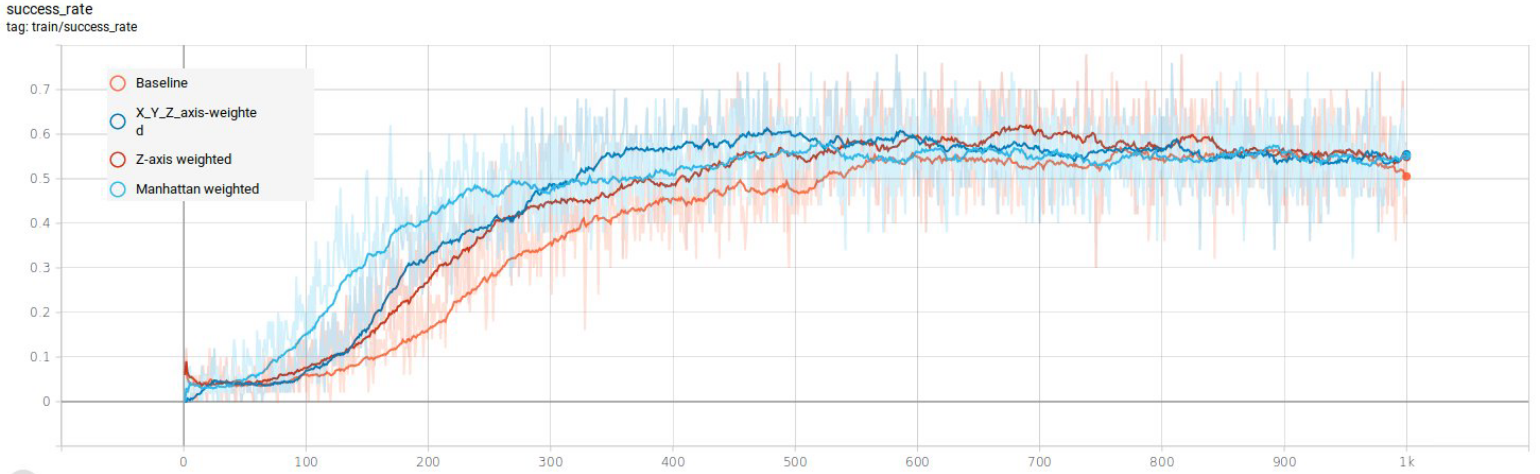
\includegraphics[width=\textwidth]{images/FPAPRRE.png}
         \caption{Success Rate Plot for Baseline 4 \cite{nagpal2020reward}.}
     \end{subfigure}
        \caption{Comparison Between Current Implementation and Baseline 4 for Fetch Pick and Place Task.}
        \label{fig:FPAPR2}
\end{figure}

The fetch reach environment is not as difficult compared to the fetch slide but presents its unique challenges as it involves complex interactions with the object and the gripper. Baseline 3 showing poor performance in the other environments does well in this task achieving a success rate of 0.8 much faster compared to the other implementations but then plateaus at the same value. On the other hand baseline 1 which was showing consistently decent performance is unable to solve this environment and achieves a success rate of 0.0. The reason is the dynamics of the environment involving the opening and closing of the grippers onto the object and then manipulating the position of the object to the goal. Baseline 3 using a randomly initialized agent with random exploration cannot just stumble onto the object with open grippers and grasp it, hence failing the task entirely. The same research has introduced ways to overcome this by using some tricks, for example, initializing the states where the gripper is already grasping the object, which converts the environment to a more reach like task and the agent is trained in this way.  Baseline 2 overcomes this problem by using demonstrations and solves the environment successfully by achieving a success rate of 0.95 in 1M time steps beating the baseline 3 with a higher success rate. Baseline 4 was also able to solve the environment successfully by just using dense rewards and achieving a max success rate of 0.6 showing that just a reward function is not enough in such complex environments. The current implementation performs better than all previous baselines by achieving a success rate of 1.0 in 310K time steps, successfully solving the environment and also providing accelerated learning. \\

\subsection{Comparison Between Demonstrations}

\begin{figure}[h!]
     \centering
     \begin{subfigure}[b]{0.4\textwidth}
         \centering
         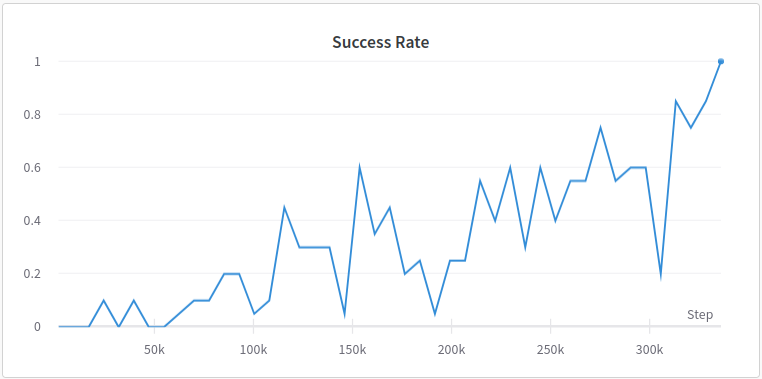
\includegraphics[width=\textwidth]{images/FPAPASR.png}
         \caption{Success Rate Plot for Current Implementation with Agent as Demonstrator.}
     \end{subfigure}
     \begin{subfigure}[b]{0.4\textwidth}
         \centering
         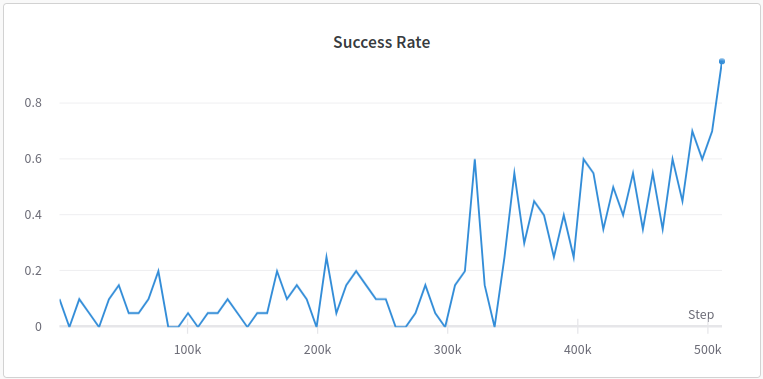
\includegraphics[width=\textwidth]{images/FPAPSSR.png}
         \caption{Success Rate Plot for Current Implementation with Script as Demonstrator.}
     \end{subfigure}
        \caption{Comparison Between Two Different Sources of Demonstrations.}
        \label{fig:CD}
\end{figure}

\begin{figure}[h!]
     \centering
     \begin{subfigure}[b]{0.4\textwidth}
         \centering
         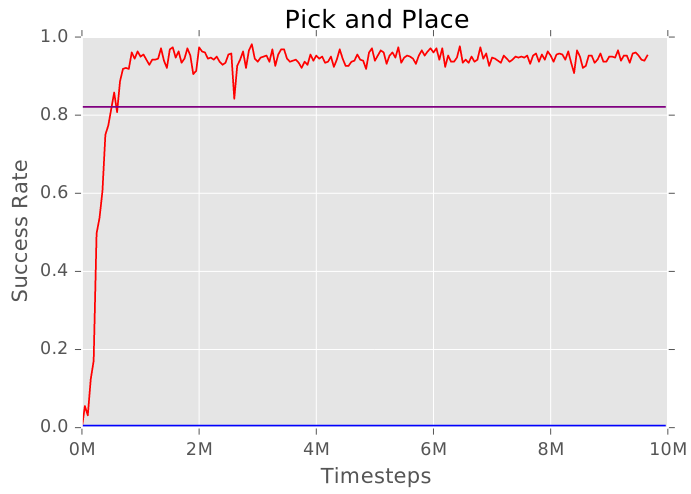
\includegraphics[width=\textwidth]{images/FPAPB.png}
         \caption{Success Rate Plot for \textcolor{blue}{Baseline 1}, \textcolor{red}{Baseline 2}, \textcolor{violet}{Baseline 3} \cite{nair2018overcoming}.}
     \end{subfigure}
     \begin{subfigure}[b]{0.4\textwidth}
         \centering
         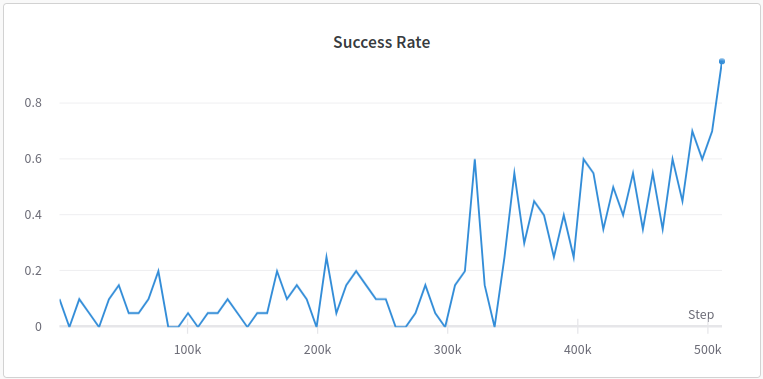
\includegraphics[width=\textwidth]{images/FPAPSSR.png}
         \caption{Success Rate Plot for Current Implementation with Script as Demonstrator.}
     \end{subfigure}
        \caption{Comparison Between Current Implementation with Different Demonstrations Source and Baselines 1, 2 and 3 for Fetch Pick and Place Task.}
        \label{fig:CDB}
\end{figure}

\begin{figure}[h!]
     \centering
     \begin{subfigure}[b]{0.4\textwidth}
         \centering
         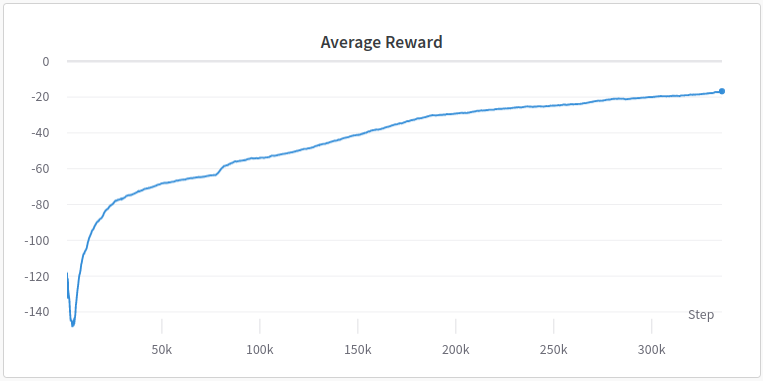
\includegraphics[width=\textwidth]{images/FPAPAAR.png}
         \caption{Average Reward Plot for Current Implementation with Agent as Demonstrator.}
     \end{subfigure}
     \begin{subfigure}[b]{0.4\textwidth}
         \centering
         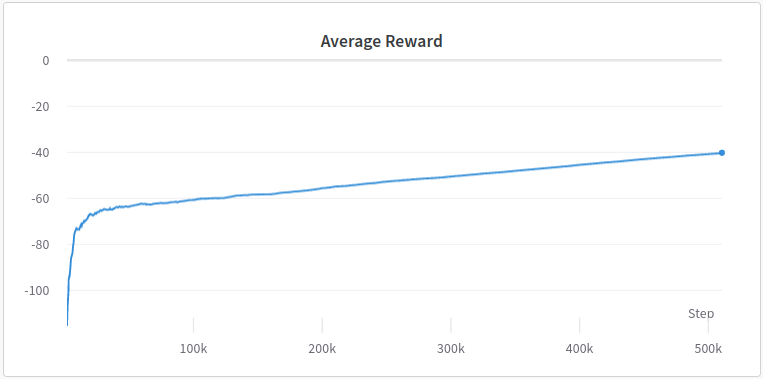
\includegraphics[width=\textwidth]{images/FPAPSAR.png}
         \caption{Average Reward Plot for Current Implementation with Script as Demonstrator.}
     \end{subfigure}
        \caption{Comparison Between Average Rewards for Different Demonstrations Sources.}
        \label{fig:CDAR}
\end{figure}

Figure \ref{fig:CD} shows the comparison between two different sources of demonstrations for the fetch pick and place environment. It is evident that even after varying the source of demonstrations the current implementation can successfully solve the environment. However, there are some interesting observations. The method using an agent as the demonstrator performs slightly better than the method that uses the handcrafted script as the demonstrator. The difference in convergence rate is not huge as a cause for concern but the noticeable difference has to be mentioned. The reason for this could be the ability of the demonstrator to complete the task and present rewards faster. On testing, it can be seen that even with external noise added the agent demonstrator can complete the task within 30 time steps out of the total 50 time steps limit per episode whereas the script takes around 40 time steps to complete the task. This delayed completion of the task could have influenced the learning agent to mimic similar behaviors as this method is behavior cloning after all. Figure \ref{fig:CDAR} shows the average reward for both the agents after a successful training session. From the figure, it can be seen that the agent which learned from the agent demonstrator has a higher average reward per episode compared to the agent which had the handcrafted script as the demonstrator. This observation further confirms the fact the slight delay in convergence time might be due to the agent mimicking the behavior of finishing the task later thus slowing down the training slightly. Even though there is a slight delay in training time between the two sources of demonstrations, both the sources can complete the task and provide accelerated learning compared to the previous baseline. \\

\subsection{Generalization Capability}

\begin{table}[h!]
\begin{tabular}{|c|c|c|}
\hline
Fetch Environment & Baseline 1 Test Success Rate & Current Implementation Test Success Rate \\ \hline
Reach          & 1.0 & 1.0 \\ \hline
Pick And Place & 0.8 & 0.9 \\ \hline
Push           & 0.8 & 0.9 \\ \hline
Slide          & 0.4 & 0.4 \\ \hline
\end{tabular}
\caption{Test Success Rate Comparison Between Current Implementation and Baseline 1.}
\label{tab:GC}
\end{table}

Table \ref{tab:GC} shows the test results of the trained agents for baseline 1 and the current implementation in all the environments. The success rates are calculated by averaging the success rate of a test set across 5 different random seeds. The current implementation can match the performance of baseline 1 in the reach and slide tasks and can outperform the baseline in the push and pick and place tasks. It can be observed that even though the current implementation can deliver good performance in the other environments it falls short in the slide task. It performs better than the baselines in training and equals the performance of the baseline in testing given the complexity of the environment this is not a bad result but definitely can be improved upon. As an extension of this research, it would be interesting to see if the transition from behavior cloning to complete reinforcement learning of the learned agent can deliver better performance. Using an agent trained using the current implementation and then using pure reinforcement learning to fine-tune the agent to try and see if it is possible to achieve better performance while still maintaining the accelerated learning. \\

\subsection{Number of Demonstrations Used}

\begin{table}[h!]
\begin{tabular}{|c|c|c|}
\hline
Fetch Environments & Demonstrations Baseline 2 & Demonstrations Current Implementation \\ \hline
Reach              & 100                     & 20                                    \\ \hline
Pick And Place     & 100                     & 40                                    \\ \hline
Push               & 100                     & 40                                    \\ \hline
Slide              & 100                     & 60                                    \\ \hline
\end{tabular}
\caption{Number of Demonstrations Used Compared to Baseline 2}
\label{tab:ND}
\end{table}

Table \ref{tab:ND} shows the number of demonstrations used for the current implementation compared to baseline 2 which uses a constant number of demonstrations for all the tasks. The current implementation can give better performance by using a lesser number of demonstrations. The number of demonstrations depends on the complexity of the task, which is the simple reach task needing only 20 demos, the average complexity environments of push and pick and place needing 40 demos, and the highly complex task of sliding needing 60 demos. The current implementation maintains the same number of demonstrations for the respective environments for both the sources of demonstrations used. If more demonstrations are available then well and good, but the current implementation can make do with lesser demons. Apart from the lesser number of demonstrations, as mentioned in the methodologies, adding external noise to the demons to replicate a more realistic approach in the collection of the demonstrations does not affect the performance of the agent, and the agent can do well with noisy demonstrations. As an extension to this research, it would be interesting to test this method with different combinations of demonstrations for example using a lesser number of high-quality demonstrations and a higher number of lower quality demonstrations. \\

\subsection{Model Complexity \textit{vs} Convergence Rate}

\begin{figure}[h!]
    \centering
    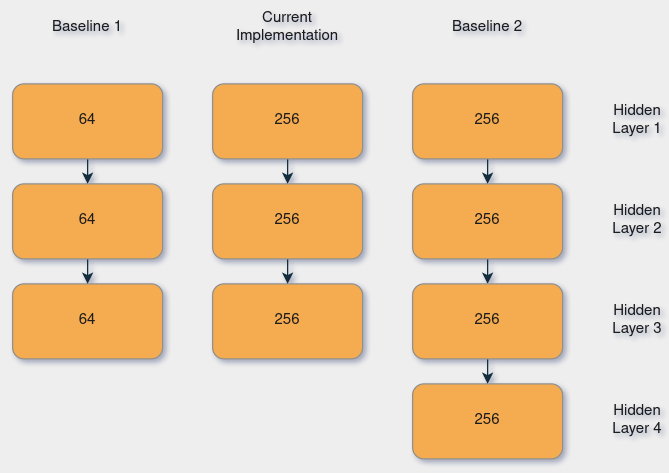
\includegraphics[width=\textwidth]{images/MAC.png}
    \caption{Model Architecture Comparison.}
    \label{fig:MAC}
\end{figure}

Figure \ref{fig:MAC} shows the comparison of the model complexity between the current implementations and the baselines. Baseline 1 was able to solve the tasks with relatively lesser model complexity of having 3 layers with 64 neurons in each layer. Both the current implementation and baseline 2 which use demos for learning have a higher model complexity, the baseline 2 having the highest of the lot with 4 layers and 256 neurons each while the current implementation has a slightly reduced version of the same with 3 layers and 256 neurons each. Baseline 1 has the highest convergence rate but the training time was reduced using powerful hardware resources, it uses no demonstrations and a random agent so it can get away with simple model complexity. Due to the use of demonstrations to prevent catastrophic forgetting of learned behaviors a higher complexity is required for baseline 2 and the current implementation, but the current implementation can perform better than the baseline 2 using a relatively lesser complex model, striking a good balance between the convergence rate and model complexity. \\

\subsection{Hardware Complexity \textit{vs} Training Time}

\begin{table}[h!]
\resizebox{\textwidth}{!}{%
\begin{tabular}{|c|ccc|ccc|ccc|}
\hline
Fetch Environment &
  Current Implementation &
   &
   &
  Baseline 1 &
   &
   &
  Baseline 4 &
   &
   \\ \hline
 &
  \multicolumn{1}{c|}{Hardware} &
  \multicolumn{1}{c|}{Training Time} &
  Success Rate &
  \multicolumn{1}{c|}{Hardware} &
  \multicolumn{1}{c|}{Training Time} &
  Success Rate &
  \multicolumn{1}{c|}{Hardware} &
  \multicolumn{1}{c|}{Training Time} &
  Success Rate \\ \cline{1-1} \cline{3-4} \cline{6-7} \cline{9-10} 
Reach &
  \multicolumn{1}{c|}{\begin{tabular}[c]{@{}c@{}}Intel i7-7th gen\\ 32Gb Ram\\ Gtx 1060 6Gb\end{tabular}} &
  \multicolumn{1}{c|}{0.1h} &
  1.0 &
  \multicolumn{1}{c|}{\begin{tabular}[c]{@{}c@{}}Distributed System\\ with 8 Parallel Workers\end{tabular}} &
  \multicolumn{1}{c|}{2.5h} &
  1.0 &
  \multicolumn{1}{c|}{-} &
  \multicolumn{1}{c|}{-} &
  - \\ \cline{1-1} \cline{3-4} \cline{6-7} \cline{9-10} 
Pick And Place &
  \multicolumn{1}{c|}{"} &
  \multicolumn{1}{c|}{3.0h} &
  1.0 &
  \multicolumn{1}{c|}{"} &
  \multicolumn{1}{c|}{2.5h} &
  0.0 &
  \multicolumn{1}{c|}{\begin{tabular}[c]{@{}c@{}}Intel i7-8th gen\\ 16Gb Ram\\ Gtx 1060 6Gb\end{tabular}} &
  \multicolumn{1}{c|}{3.0h} &
  0.6 \\ \cline{1-1} \cline{3-4} \cline{6-7} \cline{9-10} 
Push &
  \multicolumn{1}{c|}{"} &
  \multicolumn{1}{c|}{10.0h} &
  0.95 &
  \multicolumn{1}{c|}{"} &
  \multicolumn{1}{c|}{2.5h} &
  0.8 &
  \multicolumn{1}{c|}{-} &
  \multicolumn{1}{c|}{-} &
  - \\ \cline{1-1} \cline{3-4} \cline{6-7} \cline{9-10} 
Slide &
  \multicolumn{1}{c|}{"} &
  \multicolumn{1}{c|}{20.0h} &
  0.6 &
  \multicolumn{1}{c|}{"} &
  \multicolumn{1}{c|}{8h} &
  0.4 &
  \multicolumn{1}{c|}{-} &
  \multicolumn{1}{c|}{-} &
  - \\ \hline
\end{tabular}%
}
\caption{Comparison between the hardware's used between the current implementation and baselines.}
\label{tab:HC}
\end{table}

Table \ref{tab:HC} shows the hardware used by the current implementation and baseline 1 to solve the same set of tasks. Baseline 1 uses high-end hardware with a distributed system across 8 parallel workers running the environments and training the agent simultaneously. Even though the convergence rate for this baseline is higher, that is compensated by the use of powerful hardware showing more number time steps faster to the agent and solving the task with a much lesser training time. The current implementation and baseline 4 both use very modest hardware in the form of a laptop computer. The problem with baseline 4 is just a reward function is not enough for this complex environment, even though it can solve the task, the performance is just average. The current implementation using similar hardware can perform much better beating both baselines in all the tasks using modest hardware resources. It may not be the fastest in terms of training time but can deliver a low convergence rate. The agent can converge quickly with lesser interactions in the environment and seeing lesser states, striking a good balance in terms of hardware resources used and training time. \\